\documentclass[11pt]{article}
\usepackage[margin=1in]{geometry}
\usepackage{amsmath,amssymb}
\usepackage{graphicx}
\usepackage{booktabs}
\usepackage[hidelinks]{hyperref}
\usepackage{xcolor}

\newcommand{\rmean}{\langle r \rangle}
\newcommand{\statver}[1]{\textbf{#1}}

\title{Open-source finite-element tests of the Rosenzweig--Porter hypothesis
for freely vibrating plates:\\ preliminary results}
\author{J.~Arturo Ornelas Brand\\
\small Independent Researcher, Aguascalientes, M\'exico}
\date{July 3, 2026 --- draft v0.1 (companion to the ``Why Rosenzweig--Porter?'' program)}

\begin{document}
\maketitle

\begin{abstract}
The companion paper \emph{Why Rosenzweig--Porter?} proposes that the
intermediate (Rosenzweig--Porter, RP) spectral statistics observed in freely
vibrating thin plates arise from evanescent-wave coupling at free edges
acting on an integrable base, and it registers the numerical tests that would
decide the hypothesis, assigning them to COMSOL ``or finite elements''. We
report the first execution of that program with a fully open-source stack
(scikit-fem, Argyris elements, certified eigensolvers), under preregistered
readings and measurement-based accuracy gates. Main findings: (i)~the
boundary-controlled Poisson$\to$intermediate transition is confirmed at
$3.6\sigma$; (ii)~the geometry program yields a three-tier hierarchy governed
by the boundary's adaptedness to separable coordinates --- exact reduction
(disk) gives Poisson; coordinate-adapted boundaries (ellipse, sector,
rectangle) give weak sparse coupling; unadapted boundaries (triangle,
superellipse $p\neq2$) give full coupling --- with a $+12.2\sigma$ step
between the ellipse ($p=2$) and the smooth soft-cornered superellipse
($p=3$); (iii)~Gap~A, executed for the first time on the true operator,
shows $N$-independent inverse participation ratios: at accessible sector
sizes ($N\le324$) each free-plate mode is $\approx$1--2 free-free beam
products, i.e.\ sparse avoided-crossing hybridization rather than an
RP-fractal phase. The results support the free-edge coupling mechanism while
sharpening it in two ways that only true-operator computations could reveal.
All experiments, gates, and raw data are reproducible from the repository.
\end{abstract}

\section{Introduction}

L\'opez-Gonz\'alez and coworkers reported that flexural spectra of freely
vibrating rectangular plates exhibit avoided crossings and intermediate
spacing statistics within each symmetry sector, well fitted by the
Rosenzweig--Porter (RP) random-matrix model, while simply supported plates
are Poissonian~\cite{lopez2021}; the finding extends to a freely vibrating
disk sector~\cite{lopez2024comsol}. The companion hypothesis
paper~\cite{ornelas2026} formalizes a mechanism --- evanescent components of
free-edge eigenfunctions generate an inter-mode coupling $V$ on an
integrable base $H_0$ --- and registers the calculations that would support
or challenge it. This note reports the first systematic execution of those
calculations, replacing COMSOL with an open-source pipeline so that every
number can be re-derived from a commodity workstation.

Throughout, $D=\rho h=1$, eigenvalues $\Lambda=\omega^2$ of
$D\nabla^4 w = \rho h\,\omega^2 w$, and the canonical rectangle has $a=1$,
$b=1/1.6189043236$, $\nu=0.33$. Spacing-ratio statistics
$r_n=\min(s_n,s_{n+1})/\max(s_n,s_{n+1})$ are used without unfolding
(Poisson $0.3863$, GOE $0.5307$~\cite{atas2013}), always per symmetry
sector, always against \emph{finite-size baselines computed with the
identical protocol} (never asymptotic constants); the lowest ten levels per
sector are dropped.

\section{Methods and certification}

\paragraph{Stack.} Kirchhoff--Love bending energy discretized with quintic
$C^1$ Argyris triangles (scikit-fem); free edges are the natural boundary
conditions (no constraints), simply supported edges are reached through a
validated Winkler penalty $V_n+\kappa w=0$ with $\kappa=10^{10}$
($O(1/\kappa)$ error, $3\times10^{-6}$ measured against the exact SSSS
spectrum). Eigenvalues of record come from shift-invert Lanczos without
eigenvectors; eigenvectors from banded shift-invert subspace iteration with
deflation and whitened Rayleigh--Ritz projections, certified per mode by
Rayleigh-quotient matching against the eigenvalues of record and residual
gates. Symmetry labels come from mirror/rotation-character classification
with simultaneous diagonalization of reflection Grams inside near-degenerate
clusters ($\mathbb{Z}_2\times\mathbb{Z}_2$, $C_{3v}$ including exact $E$
doublets, and single-reflection variants).

\paragraph{Accuracy policy.} Statistics-grade means eigenvalue error below
$0.1\times$ the local mean level spacing for every mode used. Every
experiment runs behind gates: an exact or semi-analytic anchor where one
exists (SSSS rectangle; Lam\'e$^2$ for the simply supported triangle; the
per-$m$ Bessel $J/I$ free-disk determinant, fundamental $x^2=5.262$ vs.\
literature $\approx5.25$), two-mesh internal checks otherwise, and --- for
curved boundaries, where inscribed-polygon geometry error caps convergence
at $O(h^2)$ --- an \emph{operational} gate: the FEM disk's class-sequence
statistics must reproduce the semi-analytic Poisson control ($0.0\sigma$
agreement measured over 1600 modes; the non-smooth error component is
bounded at $1.4\times10^{-5}$ relative, $\sim$0.3\% of a sector spacing).
Readings were preregistered in each experiment's README and committed before
execution.

\section{Results}

\subsection{E2: boundary-controlled transition (supports, $3.6\sigma$)}

Sweeping the symmetric Winkler restraint from free ($\kappa=0$) to simply
supported ($\kappa\to\infty$) on the rectangle, the pooled per-sector
$\rmean$ interpolates monotonically from $0.4422\pm0.0096$ to
$0.3908\pm0.0104$ at $\sim$200 levels/sector. Both endpoints match their
finite-size baselines exactly: the SS end equals the exact-SSSS same-window
value to four decimals, and the free end matches the independent
Legendre--Ritz reference. The transition amplitude is $3.6\sigma$ above the
separable baseline (preregistered threshold $3\sigma$); no intermediate
statistics appear at nearly-simply-supported coupling
(Fig.~\ref{fig:e2}).

\begin{figure}[htb]\centering
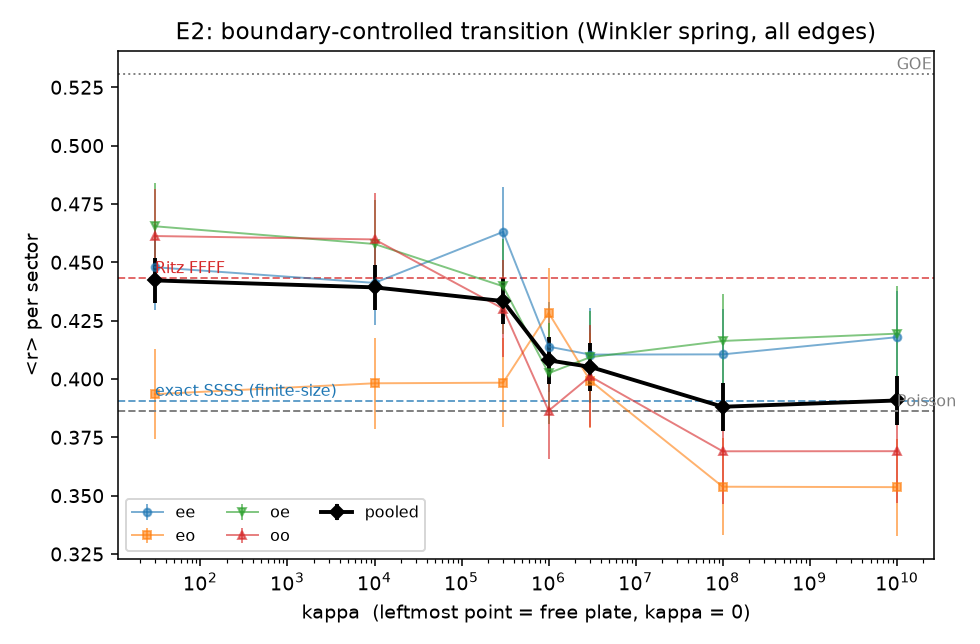
\includegraphics[width=0.72\textwidth]{figs/r_vs_kappa.png}
\caption{E2: per-sector and pooled $\rmean$ vs.\ the edge-spring constant
$\kappa$ (800 modes, Argyris $128\times80$).}
\label{fig:e2}
\end{figure}

\subsection{E3: geometry program}

\paragraph{Triangle (supports, $6.8\sigma$).} The free equilateral triangle
--- Helmholtz-integrable, biharmonically non-separable, symmetry group
$C_{3v}$ with exact $E$ doublets --- gives pooled $\rmean=0.4889\pm0.0099$
vs.\ a same-protocol simply supported baseline $0.3753\pm0.0134$ (the SS
polygon plate factorizes through the Dirichlet Helmholtz problem, i.e.\ the
Lam\'e lattice squared, matched by the FEM to $3\times10^{-5}$ across all
1000 modes). All three sectors separate positively (A$_1$ $+3.8\sigma$, $E$
$+5.6\sigma$, A$_2$ $+1.9\sigma$); 333 $E$ doublets split at
$<10^{-5}$ (Fig.~\ref{fig:e3a}).

\paragraph{Disk control (confirmed) and ellipse.} The full free disk ---
free edges with preserved separability --- is the program's zero-coupling
control: the semi-analytic class sequence gives
$\rmean=0.3905\pm0.0073$ (the companion program's executed control:
$0.386\pm0.007$), and each fixed-$m$ sequence is a picket fence. The free
ellipse ($a/b=1.6189$, area $\pi$), predicted intermediate under the naive
reading, is Poisson-consistent at 1600 modes ($0.3732\pm0.0071$); a
suggestive upward trend at 800 modes did not survive the registered
long-ladder decider (Fig.~\ref{fig:e3b}).

\paragraph{Disk sector (ambiguous, $+1.7\sigma$).} At $\theta=2.0$ rad and
800 modes the sector's two reflection classes sit $+1.2\sigma$/$+1.7\sigma$
above the disk baseline (pooled $0.4213\pm0.0095$) --- the same tendency as
the published COMSOL sector study but below our preregistered threshold; a
decisive comparison needs their mode counts ($\sim$$10^4$) or exact angles
(Fig.~\ref{fig:e3c}).

\begin{figure}[htb]\centering
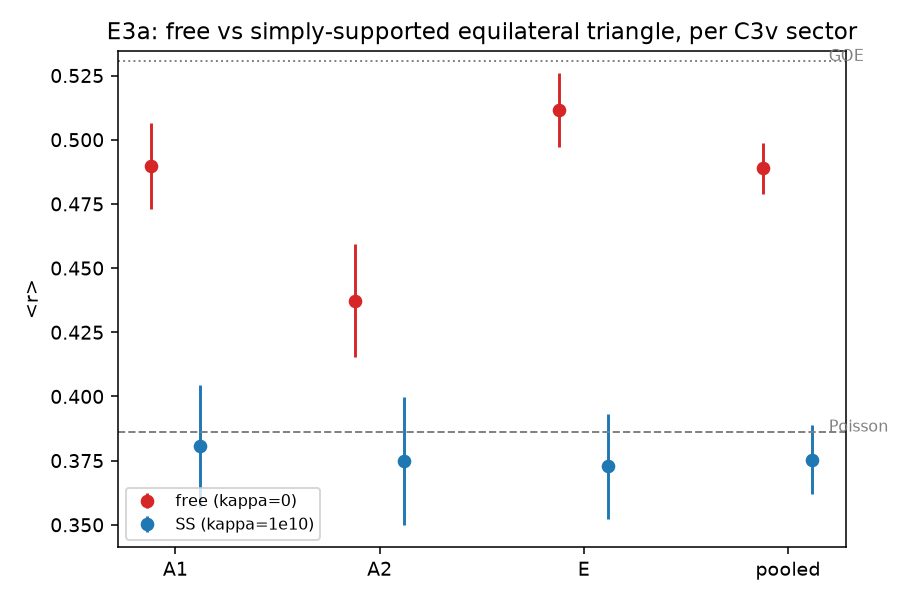
\includegraphics[width=0.55\textwidth]{figs/r_triangle.png}
\caption{E3a: free vs.\ simply supported equilateral triangle per $C_{3v}$
sector.}
\label{fig:e3a}
\end{figure}

\begin{figure}[htb]\centering
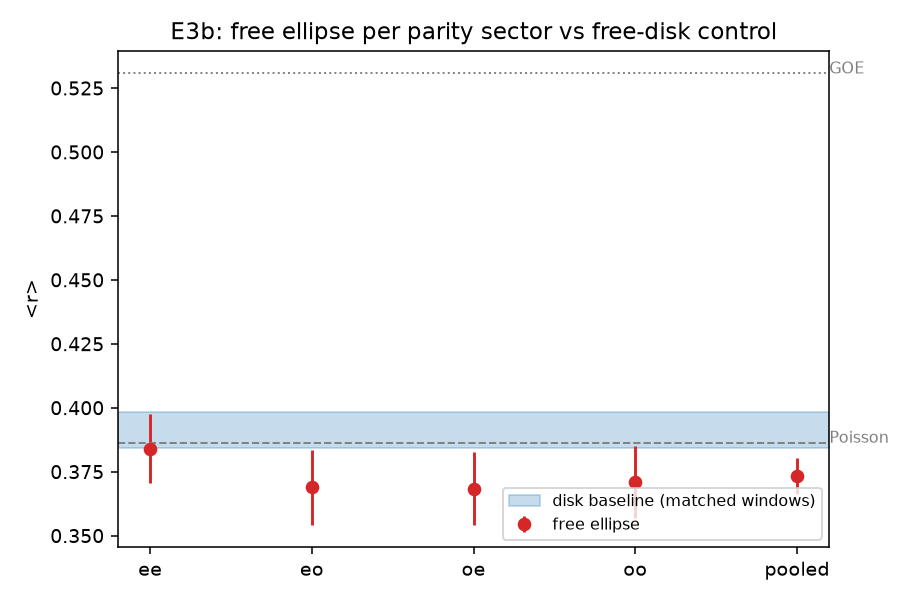
\includegraphics[width=0.55\textwidth]{figs/r_disk_ellipse.png}
\caption{E3b (v2 decider): free-ellipse parity sectors vs.\ the free-disk
control at 1600 modes.}
\label{fig:e3b}
\end{figure}

\begin{figure}[htb]\centering
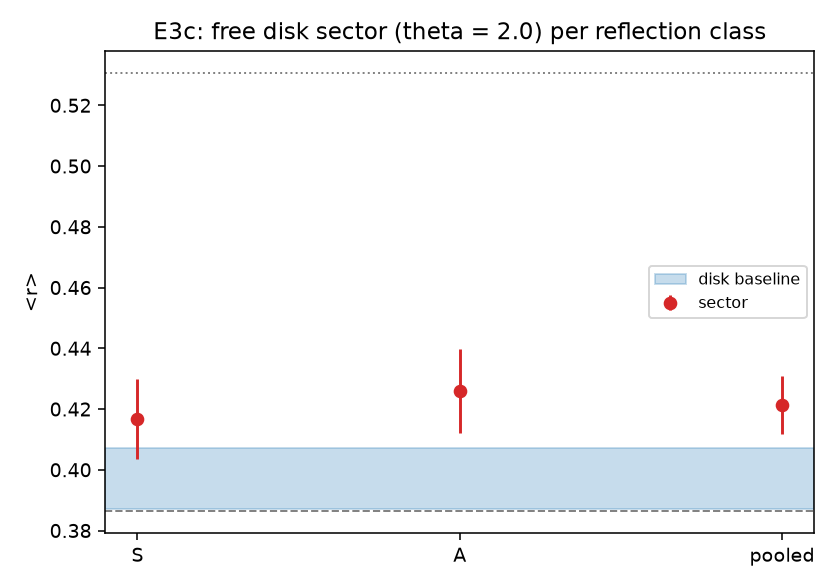
\includegraphics[width=0.5\textwidth]{figs/r_sector.png}
\caption{E3c: free disk sector ($\theta=2$) per reflection class.}
\label{fig:e3c}
\end{figure}

\subsection{E5: superellipse sweep (the discriminator)}

The family $|x/a|^p+|y/b|^p=1$ breaks biharmonic separability equally for
every $p$ while corner-region curvature grows with $p$ at fixed
$C^\infty$ smoothness. The measured sequence,
\[
\rmean(p) = 0.3732,\; 0.4944,\; 0.4893,\; 0.4942,\; 0.5159
\quad (p = 2, 3, 4, 6, 10),
\]
is a $+12.2\sigma$ \emph{step} between $p=2$ and $p=3$, a flat plateau
through $p=6$, and a mild $+2.3\sigma$ rise at $p=10$
(Fig.~\ref{fig:e5}); the statistics are refinement-stable at $0.1\sigma$
for both the headline and worst-corner points. Neither preregistered shape
(curvature-graded; true-corner threshold) fits: the operative variable is
the boundary's compatibility with separable coordinates --- the ellipse is
the family's unique quasi-separable member (confocal boundary $=$
elliptic-coordinate line) --- and corners are secondary.

\begin{figure}[htb]\centering
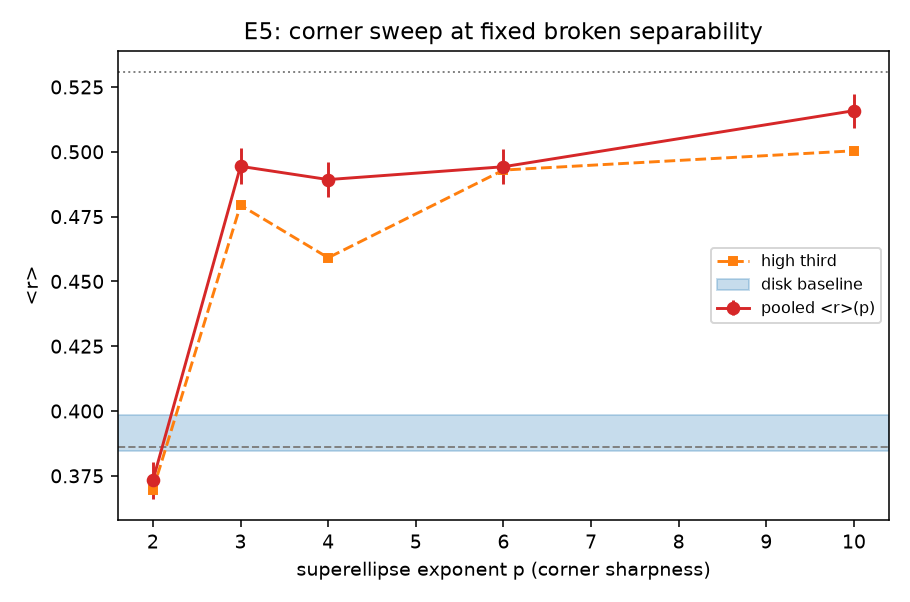
\includegraphics[width=0.62\textwidth]{figs/r_vs_p.png}
\caption{E5: $\rmean(p)$ along the superellipse family at 1600 modes per
geometry.}
\label{fig:e5}
\end{figure}

\subsection{E4: Gap A on the true operator (localized-leaning at $N\le324$)}

The companion paper's decisive test: eigenvector statistics per sector, in
the two registered representation bases (simply supported sine products and
free-free beam products), against empirical GOE baselines at identical $N$
(the T1 audit protocol). On 1200 certified eigenpairs (vector residuals
$\le8\times10^{-6}$), the mean window IPR is \emph{independent of} $N$
across the ladder $N=64$--$324$ in both bases (ladder
$D_2\approx0.02$--$0.13$; GOE $\approx1$), and in the beam basis --- which
represents the true modes with captured norm $0.999$--$1.000$ --- each mode
is $\approx$1--2 beam products (IPR $\approx0.7$;
Fig.~\ref{fig:e4}). Per the preregistered dichotomy this is the
localized/banded side at accessible $N$: sparse strong pair-hybridizations
(microscopically, the observed avoided crossings) produce intermediate
spacing statistics without RP-fractal eigenvectors. Two sharpenings:
the true-operator $D_2$ is \emph{lower} than the Ritz-model values (beam
fixed-$N$ $0.25$ vs.\ $0.35$--$0.42$), i.e.\ the model route overestimates
coupling density; and since the effective coupling grows with mode index
(E2, E3b), the verdict could still flip at the registered $N\sim2048$ rung,
reachable via quarter-plate reduction. $\Sigma^2(L\le5)$ is intermediate,
mildly below Poisson; larger $L$ is unfolding-limited.

\begin{figure}[htb]\centering
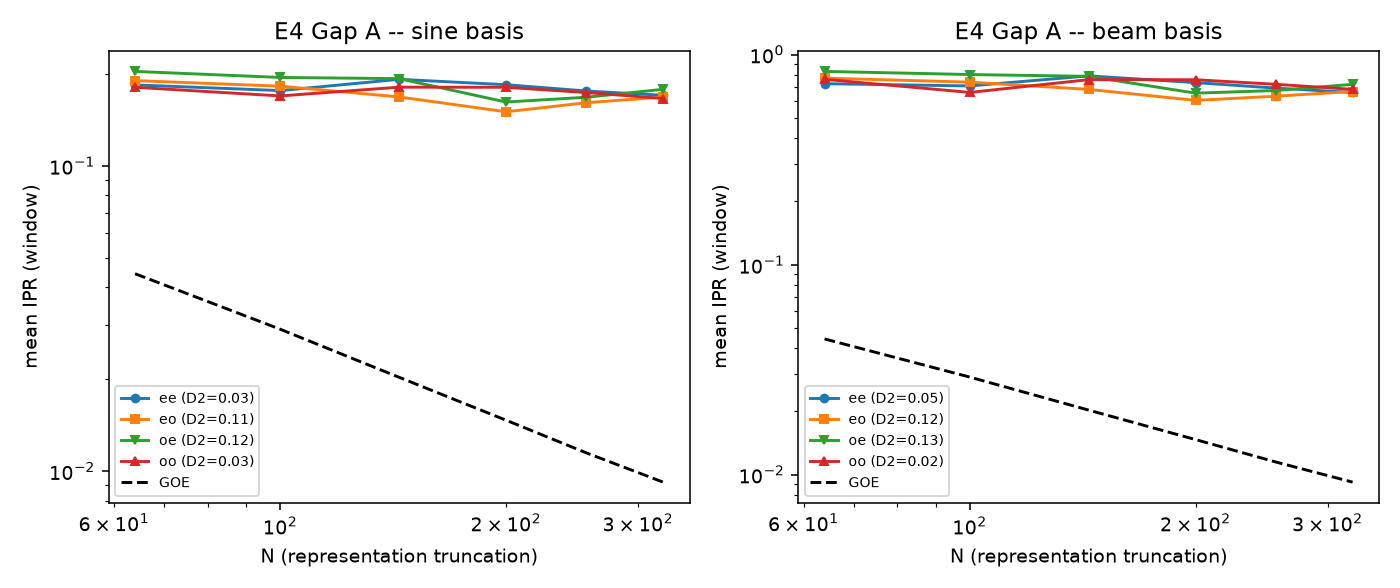
\includegraphics[width=0.95\textwidth]{figs/ipr_ladders.png}
\caption{E4: window-mean IPR vs.\ representation truncation $N$, per sector,
in the sine (left) and beam (right) registered bases, with GOE baselines.}
\label{fig:e4}
\end{figure}

\section{Synthesis}

Seven geometries fall on one hierarchy:
\begin{center}
\begin{tabular}{lll}
\toprule
tier & geometries ($\rmean$ at matched ladders) & mechanism state\\
\midrule
exact reduction & disk $0.391$ & no coupling (Poisson)\\
coordinate-adapted & ellipse $0.373$; sector $0.421$; rectangle $0.44$ &
weak, sparse coupling\\
unadapted & triangle $0.489$; superellipse $p\neq2$: $0.49$--$0.52$ &
full coupling\\
\bottomrule
\end{tabular}
\end{center}
The free-edge origin of the coupling is confirmed directly (E2). What the
data refine is the \emph{selector}: not corners, not curvature, but whether
the boundary is adapted to a separable structure of the fourth-order
operator --- with the rectangle's ``quasi-separability in the beam basis''
(E4: modes $\approx$ single beam products) unifying the picture. At
accessible mode numbers the coupling acts as sparse resonant hybridization
(avoided crossings), not yet as the dense non-ergodic RP phase; whether the
RP phase develops at higher rungs is the single most consequential open
computation.

\section{In execution and pending registered tests}

In execution at the time of this draft: \textbf{E6} (designed contact
coupling --- the companion's contact test built directly from certified
mode-shape values at contact points, plus an inverse-design demonstration of
the control law $V_{ij}=\kappa\sum_k\phi_i(x_k)\phi_j(x_k)$: post placement
and stiffness computed in closed form for a target hybridization) and
\textbf{E7} (Protocol~A mixed boundary configuration; $\rmean(\nu)$ material
independence). Pending, registered in the research plan: the annulus control
(semi-analytic); Mindlin--Reissner thick plates; $D_q$ flatness and
form-factor rival exclusion (power-law banded family) on the
strongest-coupling geometries; Gap~A at $N\sim2048$ via quarter-plate
reduction; the sector at the published study's exact angles; and comparison
against the measured aluminum-plate spectra of Ref.~\cite{lopez2021}.

\section{Reproducibility}

All experiments live in \texttt{experiments/eNN\_*} of the private
repository \texttt{plates-rp-fem} with frozen code, preregistered README,
RESULTS, raw JSON, and figures; the shared machinery is the
\texttt{platefem} package (conda env \texttt{plates-fem}: Python 3.12,
scikit-fem 12.0.2, SciPy 1.18). Total compute for E1--E5: under 8 hours on
one 8-core desktop (Ryzen 7 5800XT, 64 GB). Two numerical contributions may
be of independent use: a certified eigenpair pipeline that works around a
SciPy 1.18 shift-invert eigenvector-path failure on ill-conditioned
$C^1$-element matrices, and the measured $\sim10^{-4}$ round-off floor of
high-order Legendre--Ritz assembly for the free plate (non-monotone in basis
size beyond $\sim$96 functions/axis).

\begin{thebibliography}{9}
\bibitem{lopez2021} M.~L\'opez-Gonz\'alez et al., avoided crossings and
intermediate statistics in free rectangular plates (2021); resonant acoustic
spectroscopy with mode-shape mapping.
\bibitem{lopez2024comsol} M.~L\'opez-Gonz\'alez et al., \emph{Discovery of
avoided crossings in plate vibrations using COMSOL}, COMSOL Conference 2024
Boston.
\bibitem{ornelas2026} J.~A.~Ornelas Brand, \emph{Why Rosenzweig--Porter?
Evanescent Coupling and a Random Matrix Hypothesis for Intermediate
Statistics in Freely Vibrating Plates}, Zenodo (v4 series, 2026).
\bibitem{atas2013} Y.~Y.~Atas, E.~Bogomolny, O.~Giraud, G.~Roux,
Phys.\ Rev.\ Lett.\ \textbf{110}, 084101 (2013).
\bibitem{kravtsov2015} V.~E.~Kravtsov, I.~M.~Khaymovich, E.~Cuevas,
M.~Amini, New J.\ Phys.\ \textbf{17}, 122002 (2015).
\bibitem{leissa1969} A.~W.~Leissa, \emph{Vibration of Plates}, NASA SP-160
(1969).
\end{thebibliography}

\end{document}
